\documentclass[landscape,letter]{article}
\usepackage[fontsize=12pt]{scrextend}
\usepackage[utf8]{inputenc}
\usepackage[ngerman]{babel}
\usepackage[dvipsnames]{xcolor}
\usepackage{tikz}
\usetikzlibrary{shapes,positioning,arrows,fit,calc,graphs,graphs.standard}
\usepackage[nosf]{kpfonts}
\usepackage[t1]{sourcesanspro}
%\usepackage[lf]{MyriadPro}
%\usepackage[lf,minionint]{MinionPro}
\usepackage{multicol}
\usepackage{wrapfig}
\usepackage[top=0mm,bottom=1mm,left=0mm,right=1mm]{geometry}
\usepackage[framemethod=tikz]{mdframed}
\usepackage{microtype}
\usepackage{listings}

\let\bar\overline

\definecolor{myblue}{cmyk}{1,.72,0,.38}

\def\firstcircle{(0,0) circle (1.5cm)}
\def\secondcircle{(0:2cm) circle (1.5cm)}

\colorlet{circle edge}{myblue}
\colorlet{circle area}{myblue!5}
\definecolor{rred}{HTML}{b61010}
\tikzset{filled/.style={fill=circle area, draw=circle edge, thick},
    outline/.style={draw=circle edge, thick}}

\pgfdeclarelayer{background}
\pgfsetlayers{background,main}

\everymath\expandafter{\the\everymath \color{myblue}}
\everydisplay\expandafter{\the\everydisplay \color{myblue}}

\renewcommand{\baselinestretch}{.8}
\pagestyle{empty}

\global\mdfdefinestyle{header}{%
linecolor=gray,linewidth=1pt,%
leftmargin=0mm,rightmargin=0mm,skipbelow=0mm,skipabove=0mm,
}

\newcommand{\header}{
	\mdfsetup{%
		middlelinecolor=black,
		middlelinewidth=2pt,
                backgroundcolor={rred},
		%roundcorner=10pt}
	}
\begin{mdframed}[style=header]
\footnotesize
\sffamily
%\colorbox{yellow}

{COMP 302 Crib Sheet}\\
by~{Julian Lore}~Side \thepage \ of 1
\end{mdframed}
}

\makeatletter
\renewcommand{\section}{\@startsection{section}{1}{0mm}%
                                {.2ex}%
                                {.2ex}%x
                                {\color{myblue}\sffamily\small\bfseries}}
\renewcommand{\subsection}{\@startsection{subsection}{1}{0mm}%
                                {.2ex}%
                                {.2ex}%x
                                {\sffamily\bfseries}}



\def\multi@column@out{%
   \ifnum\outputpenalty <-\@M
   \speci@ls \else
   \ifvoid\colbreak@box\else
     \mult@info\@ne{Re-adding forced
               break(s) for splitting}%
     \setbox\@cclv\vbox{%
        \unvbox\colbreak@box
        \penalty-\@Mv\unvbox\@cclv}%
   \fi
   \splittopskip\topskip
   \splitmaxdepth\maxdepth
   \dimen@\@colroom
   \divide\skip\footins\col@number
   \ifvoid\footins \else
      \leave@mult@footins
   \fi
   \let\ifshr@kingsaved\ifshr@king
   \ifvbox \@kludgeins
     \advance \dimen@ -\ht\@kludgeins
     \ifdim \wd\@kludgeins>\z@
        \shr@nkingtrue
     \fi
   \fi
   \process@cols\mult@gfirstbox{%
%%%%% START CHANGE
\ifnum\count@=\numexpr\mult@rightbox+2\relax
          \setbox\count@\vsplit\@cclv to \dimexpr \dimen@-1cm\relax
\setbox\count@\vbox to \dimen@{\vbox to 1cm{\header}\unvbox\count@\vss}%
\else
      \setbox\count@\vsplit\@cclv to \dimen@
\fi
%%%%% END CHANGE
            \set@keptmarks
            \setbox\count@
                 \vbox to\dimen@
                  {\unvbox\count@
                   \remove@discardable@items
                   \ifshr@nking\vfill\fi}%
           }%
   \setbox\mult@rightbox
       \vsplit\@cclv to\dimen@
   \set@keptmarks
   \setbox\mult@rightbox\vbox to\dimen@
          {\unvbox\mult@rightbox
           \remove@discardable@items
           \ifshr@nking\vfill\fi}%
   \let\ifshr@king\ifshr@kingsaved
   \ifvoid\@cclv \else
       \unvbox\@cclv
       \ifnum\outputpenalty=\@M
       \else
          \penalty\outputpenalty
       \fi
       \ifvoid\footins\else
         \PackageWarning{multicol}%
          {I moved some lines to
           the next page.\MessageBreak
           Footnotes on page
           \thepage\space might be wrong}%
       \fi
       \ifnum \c@tracingmulticols>\thr@@
                    \hrule\allowbreak \fi
   \fi
   \ifx\@empty\kept@firstmark
      \let\firstmark\kept@topmark
      \let\botmark\kept@topmark
   \else
      \let\firstmark\kept@firstmark
      \let\botmark\kept@botmark
   \fi
   \let\topmark\kept@topmark
   \mult@info\tw@
        {Use kept top mark:\MessageBreak
          \meaning\kept@topmark
         \MessageBreak
         Use kept first mark:\MessageBreak
          \meaning\kept@firstmark
        \MessageBreak
         Use kept bot mark:\MessageBreak
          \meaning\kept@botmark
        \MessageBreak
         Produce first mark:\MessageBreak
          \meaning\firstmark
        \MessageBreak
        Produce bot mark:\MessageBreak
          \meaning\botmark
         \@gobbletwo}%
   \setbox\@cclv\vbox{\unvbox\partial@page
                      \page@sofar}%
   \@makecol\@outputpage
     \global\let\kept@topmark\botmark
     \global\let\kept@firstmark\@empty
     \global\let\kept@botmark\@empty
     \mult@info\tw@
        {(Re)Init top mark:\MessageBreak
         \meaning\kept@topmark
         \@gobbletwo}%
   \global\@colroom\@colht
   \global \@mparbottom \z@
   \process@deferreds
   \@whilesw\if@fcolmade\fi{\@outputpage
      \global\@colroom\@colht
      \process@deferreds}%
   \mult@info\@ne
     {Colroom:\MessageBreak
      \the\@colht\space
              after float space removed
              = \the\@colroom \@gobble}%
    \set@mult@vsize \global
  \fi}

\makeatother
\setlength{\parindent}{0pt}

\begin{document}
\small
\begin{multicols*}{5}
  \color[HTML]{11114E}
\section{Uninformed Search}
\paragraph{Search Problem} \textbf{State space} $S$: all possible configs of
domain, \textbf{initial state} $s_0 \in S$ (start state), \textbf{goal
states} $G \subset S$ (end states), \textbf{Operators} $A$ (actions
avail), \textbf{Path}, \textbf{Path cost}, $c$, \textbf{Solution} of
search problem: path from $s_0$ to $s_g\in G$, \textbf{Optimal
  solution}: path with min \$
\\ Eight puzzle: States (conf of puzzle), goals (target conf), ops
(swap blank with adj), path cost (\# moves)
% \\ Basic assumptions for now: (static, observable, deterministic env,
% discrete states)
\\ Represent state space search as graph, vertices are states, edges
are operators. Build \textbf{search tree} to find goal
state. \underline{Search tree nodes not same as graph nodes}
\\ Data struct for search tree: \textbf{Node} (state id, parent state
+ op, cost of path, depth. To expand node, apply all legal ops and gen
new nodes.
\paragraph{Generic search alg} Init search tree with $s_0$. Loop: If
no nodes can be expanded, fail. Else choose node to expand, if node
has goal, return path, else expand node by applying each op and
getting new states, adding to tree.
\paragraph{Uninformed (blind) search} If state isn't goal, you \colorbox{red}{don't
know how close} to goal it might be.
\paragraph{Uninformed Search algs}
\colorbox{yellow}{Key props}:  \textbf{Completeness} (guarantee soln if it exists),
\textbf{Optimality} (how good is soln), \textbf{space complexity},
\textbf{time complexity}.
\subparagraph{Search complexity} \textbf{Branching factor} $b$,
\textbf{solution depth} $d$
\\ All uninf search time complex $O(b^d)$, very general and very
expensive, no knowledge.
\\ \textbf{Breadth-first search} (\colorbox{yellow}{complete} w/ finite $b$, guaranteed
shortest path if unit cost = \colorbox{yellow}{optimal}, but not if
weighted graph). \colorbox{yellow}{$O(b^d)$} space. \textbf{depth-first
  search} (\colorbox{yellow}{$O(bm)$} space, easy to do recursively, more efficient than
BFS if many goal paths, \colorbox{yellow}{\textbf{not optimal}}, may not complete
(cycles), don't use DFS for big $d$), \textbf{uniform-cost search}
(BFS but with \textbf{general} (weighted graph) step costs, use a
pqueue, \colorbox{yellow}{opt \& comp}), \textbf{depth-limited search} (DFS but stop at goal or max
depth, always terms, but \colorbox{red}{not complete}),
\textbf{iterative deepening search}(depth-lim search but increasing
depth, expands nodes mult times, \colorbox{yellow}{complete}, \colorbox{yellow}{linear mem req} like DFS,
but more time, \colorbox{yellow}{optimal} if unit cost, preferred for large state spaces)
\\ Revisiting states: maintain \textbf{closed list} to store expanded
nodes, good for probs with repeated states. $O(|S|)$ time and
space. Sometimes re-expanding states could be better (compare old and
new path cost, also sometimes domain may be too large to store all
states).
\\ \colorbox{yellow}{What method to use?} To find opt: BFS, IDS for unit cost,
uniform-cost search if general cost. Large state space: DFS max length
is known, IDS otherwise. Limited mem: DFS/IDS. Quickly find best soln
with budget: Depth-limited if unit cost, UCS if gen cost.
\color{Orange}
\section{\textcolor{Orange}{Informed Search}} Use \textbf{heuristics} to guide search. Uninformed
expand nodes based on dist from start node. Informed expands based on
\textbf{distance to goal}. If we don't know exact distance, we use
intuition, \textbf{heuristic}. Heuristics come from prior knowledge of
prob, exact soln to \colorbox{yellow}{relaxed vers} of prob, learning from exp
\\ Heuristic for path planning: straight-line distance between two places.
\\ Eight puzzle: number of misplaced tiles, total Manhattan dist
\paragraph{Algs} \textbf{Best-First Search}(\colorbox{yellow}{greedy}, expand most
promising node first, close to BFS, if heuristic is 0, then same as
BFS, opp of UCS(cost-so-far) vs cost-to-go, $O(b^d)$ time/space, good
heuristic can make $O(bd)$, \textbf{not always complete}(loops), but
complete if finite space if we check repeated, not optimal), \textbf{Heuristic
  Search}(Problem: best-first 
too greedy, doesn't account for cost so far. Soln: \textbf{Heuristic
  search}, greedy wrt to $f = g+h$, where $g$ is cost so far, $h$ is
heuristic. Use pq, add to q w/ p: $f = g + h$, end when goal popped
from q. Note we continue expanding nodes after finding goal if
$\exists$ unexpanded w/ lower cost than current path to goal. Not
optimal, unless we put conditions on heuristics),
\textbf{A* Search} (Heuristic search with AH. Complete,
$f(s)=g(s)+h(s)\leq g(s)+c(s,s')+h(s')=f(s')$ by consistency, so no
node can be re-expanded. If soln, c must b bounded, so $A*$ will
find. Optimal, prove by contradiction, showing impossible that subopt
goal is expanded before opt. Still worst case $O(b^d)$, but $O(bd)$
with perfect heuristic because only expand nodes on opt path. With
given $h$, no other search alg can expand less nodes),
\textbf{Iterative Deepening A*}(DFS, but use $f$ to determine order to
explore children instead of depth. Same props as $A*$, but less
mem. If we remember expansion of old nodes $\to$ SMA*)
\paragraph{Admissible heuristics} $h^*(n)$ is shortest p from $n$ to
any goal. $h$ is \textbf{admissible heuristic} if $h(n) \leq h^*(n)
\forall n$. They are optimistic. Trivial ah: $h(n)=0 \forall n$, get
UCS. Obviously $h(g)=0 \forall g \in G$ for AH. Usually relaxed vers
of prob gives AH.
\paragraph{Consistency} AH $h$ is called \textbf{consistent/monotone*}
if for every state $s$ and succ $s'$, $h(s) \leq c(s,s') + h(s')$,
i.e. $h$ gets more precise as we get closer to goal. Vers of triangle
ineq. Can fix inconsistent heuristics by: $f(s')=g(s')+h(s') \to
f(s')=\max\{g(s')+h(s'),f(s)\}$
\paragraph{Dominance} $h_2(n) \geq h_1(n) \forall n$ and both AH, then
$h_2$ dominates $h_1$, i.e. more informative.
\paragraph{Decomposition} Break complex prob into smaller
parts. Decomp and putting soln together may give up optimality. Use
decomp for probs we can't solve w/o. Subsolns can be cached \&
reused. Need to be careful that when we chose subgoal, overall prob
still has soln. \textbf{Macro-action} is sequence of actions from orig problem
(e.g. make T for Rubik's)
\\ \textbf{Abstraction} ignores info to speed up comp, make compact
representation, map several real states to one abstract state
\color[HTML]{008080}
\section{\textcolor[HTML]{008080}{Optimization}}
Typically large continuous/combinatorial state space. Can't search all
possible soln. Non-uniform cost.
\paragraph{Traveling salesman prob} Vertices+dist between pairs. Get
shortest path to visit each vert once. Tour = path that satisfies
goal.
\\ Optimization prob described by \textbf{states} and
\textbf{evaluation function}, note that states are candidate solutions
(can be partial or wrong)
here, \colorbox{red}{not description of world}. Func corresponds to
path cost.
\paragraph{Optimization Search}
\textbf{Constructive methods}, start from scratch and build
up. \textbf{Iterative improvement}, start with soln, improve. Both
involve \colorbox{green}{local} search.
\paragraph{Generic local search}
Start at init $X_0$, repeat until satisfied: Gen neighbors of $X_i$;
eval them. Select one of the neighbors $X_{i+1}$ to become current
config.
\paragraph{Discrete Hill-Climbing}Start with $X_0$, val $E(X_0)$. Gen
neighbors of $X$ and $E(X_i)$. Get $\max_i E(X_i)$. If this max is
less than $E_{\max x}$ of init, then return. Else update $X$ to be new $X_i$
and $E$ to be new $E_{\max}$. This is a variant of best-first search,
easy to prog, no memory of past req, can handle large probs. Small
neighborhood = less neighbors, possibly worse soln, large
neighborhood = more to eval, possibly less local optima, better
soln. \colorbox{red}{Problem:} hill climbing can easily get stuck in
plateau or local opt, to fix, use random re-starts or pick any move
that leads to improvement (\textbf{randomize hill climbing}).
\paragraph{Simulated annealing} Like hill climbing, but allows bad
moves to escape local opt. Decrease size+freq of bad moves over
time. \\Alg: Start with $X_0$ and $E(X_0)$. Loop until satisfied:
choose random neighbor, if val is greater than $E_{max}$, replace
current max. If greater than current val we holding, replace current
$X$. Else, with prob $p$, still replace cur val. Return max at end.
\\ What to use for $p$? Constant, val that decays to $0$, val that
depends on how bad move is. We usually use \colorbox{green}{Boltzmann
  distribution}$\mathbf{p = e^{-(E-E_i)/T}}$, bad $E_i \to $small
$p$. T here is called \textbf{temperature}, usually start high then
decrease to 0 over time. Can decrease $T$ by mult by constant $0 <
\alpha < 1$ at every iter. If T is high $\to$ alg is in exploratory
phase, if low, exploitation phase.
\\ If T decreases ``slowly enough'', \colorbox{green}{optimal}, but
may take $\infty$ moves. SA better than HC when lots of local opt. HC
preferred if func is smooth, not many local opt, most local opt are
similar.
\paragraph{Parallel search} Run mult separate searches (HC or SA) in
parallel, keep best soln
\paragraph{Local beam search} Like parallel search, but share info
across searches. Start $k$ searches in parallel, but keep $k$
(\textbf{beam width}) top
solns at each step.
\paragraph{Genetic algs} \textbf{Individual}=candidate soln. Each
indiv has \textbf{fitness} (quality of soln). \textbf{Population} =
set of indivs. Pops change over \textbf{generations} by applying
\textbf{operations}(mutation(inject random change with mutation rate =
prob of mutation occur)/crossover(combine parts of indivs to make new
indiv, use \textbf{crossover mask} to specify which parts taken from 1
indiv as bin string, rest taken from other)/selection) to indivs. Higher
fitness = more likely to survive \& reproduce. Usually represent
indivs by \textbf{binary string}.
\\ \colorbox{yellow}{Alg}: (params: fitness,threshold,p,r,m) \underline{init} $P$ with
$p$ rand indivs. \underline{Eval}, get Fitness(h) $\forall h \in
P$. While $\max_h Fitness(h)<threshold$: Select $(1-r)p$ members of
$P$ to put in $P_s$. Crossover $\frac{rp}{2}$ pairs of indivs. For
each pair, produce two offspring and incl in $P_s$. Mutate 1 rand bit
in $mp$ rand indivs of $P_s$. Update $P \gets P_s$. Eval fitness
$\forall h \in P$.
\paragraph{Selection} Survival of fittest: \textbf{Fitness
  proportionate}, might lead to crowding (mult copies of same soln),
\textbf{tournament selection}, pick 2 rand indivs, with prob $p$
select fitter one. \textbf{Rank selection}, sort all by fitness, prob
of selection proportional to rank. \textbf{Softmax (Boltzman)
  selection}
$P(i)=\frac{e^{Fitness(i)/T}}{\sum_{j=1}^{P}e^{Fitness(j)/T}}$.
\\ \colorbox{yellow}{Elitism}, best soln can die during evol, so we
preserve best soln encountered. Genetic algs more expensive than HC \&
SA.
\paragraph{Pros cons of gen alg} \colorbox{green}{Pro:} Intuitive due to analogy, can be
effective if tuned properly. \colorbox{red}{Bad:} Perform dependent on
encoding of problem. Many params to tweak. Low mutation rate =
overcrowding. Too high = too random.
\color[HTML]{ff7373}
\section{Constraint Satisfaction Problems} Use constraints to
\colorbox{green}{narrow} search space. Def: \textbf{variables} $V_i$
that can take vals from domain $D_i$. \textbf{Constraints} specifying
allowed combinations of values for variables. Constraints can be
represented as a function or list of allowable vals. \textbf{CSP
  solution} is assignment of vals to vars st all constraints
true. Usually want to find \underline{any soln} or find that no soln
exists.
\paragraph{Approaches}
\textbf{Constructive approach}, state = vals assigned so far. Use
\colorbox{green}{forward search} to fill soln. Gen purpose, works for
all CSPs. \textbf{Random approach}, start with broken complete assn of
vals to vars. Fix broken constrs by re-assign vars. Use optimization.
\paragraph{Problem def}\textbf{State} (vals assigned so far, can be
partial/inconsistent). \textbf{Initial state} (all vars
unassgn). \textbf{Operators} (assign val to unass var). \textbf{Goal
  test} = all vars assigned, no constraint false, complete and
consistent assignment. Problem is
\colorbox{green}{deterministic}. Note that \colorbox{yellow}{depth is
  limited to \# of vars}, can use DFS or depth-limited search.
\\ Uninformed search for map coloring: choose unassigned var, assign a
val. This is complete and optimal, but complexity is worst possible,
$n! d^n$, ($n$ vars, $d$ vals). Branching factor \colorbox{red}{very
  high}. Var assgnment order irrelevant, many paths equiv.
\paragraph{Constraint graph}Nodes are vars, \colorbox{green}{arcs}
show constraints. Can use graph struct to accelerate search. Use
\textbf{inference} to reduce search
space. \colorbox{green}{pre-process} graph to remove
inconsistencies. Var is \textbf{arc-consistent} if all val in domain
satisfies vars binary constraints. Network is \textbf{generalized
  arc-consistent} if all vals in domain of all vars are all
arc-cons. \colorbox{yellow}{Keep applying arc-consistency} until no
changes to get generalized arc-cons.
\paragraph{Ex} Map coloring: vars = countries, domains = r,g,b,
constraints = adj countries cannot be same color, $C_1 \neq C_2
\ldots$.
\\ 4 queens: 1 queen/col, vars = $Q_1, \ldots$, row of each
queen. Domain = ${1,2,3,4}$. Constraints: $Q_i \neq Q_j$ (not same
row), $|Q_i-Q_j| \neq |i-j|$ (not same diag)
\paragraph{Backtracking search} DFS but fix order of var assn $b =
|D_i|$. If no assignment for specific var, backtrack to prev var and
try diff val. Basic uninformed alg.
\paragraph{Forward checking} Keep track of legal vals for unassigned
vars. When you assign vars, look at unassigned vars connected via
constraint and delete from their domain any inconsistent vals to new
assgn.
\paragraph{Heuristics for CSP} For selecting vars:
\textbf{minimum-remaining vals} = choose var that is most
constrained \colorbox{green}{more info} if one branch is not
satisfiable ($1/2$ of branches bad vs $1/100$ branches bad). \textbf{Degree heuristic} = choose var that imposes most
constraints on remaining vars, can use to break ties from min-remain
vals heuristic. To select a val: \textbf{least-constraining val}:
assign a val that rules out fewest vals for other vars
(\colorbox{green}{less chance of conflict} in future).
\\ Worst-case $d^n$. Tree structured constraint graph gives
$O(nd^2)$. Nearly-tree structured: $O(d^c(n-c)d^2)$ using
\textbf{cutset conditioning}, find vars st removing them turns graph
into tree. Instantiate them all possible ways, $c$ is size of cutset.
\paragraph{Local search} \textbf{Iterative improvement alg} Start with
broken but complete assnment of vals \& vars. Allow var assgns that
don't satisfy some constraints. Randomly select conflicted vars. Ops
reassign var vals. \textbf{min-conflict heuristic} chooses val that
violates fewest constraints. This is hill climbing.
\color[HTML]{8b0000}
\section{Uncertainty} Actions may be
\textbf{non-deterministic}. Problems can be \textbf{(fully) observable},
\textbf{partially observable} or \textbf{non-observable}.
\paragraph{Searching under uncert} Cannot determine future states in
advance (i.e. depend on die roll). Soln is not path, but
\textbf{contingency plan/strategy}.
\\ Vacumm ex. Two rooms, vacuum in one of the rooms, rooms can be
dirty or clean. When non-observable, need plan. What states possible
after doing an action? Reason over \textbf{beliefs} (sets of
states). \colorbox{green}{Total \# possible beliefs} = power set of
all states w/o empty. Less \colorbox{yellow}{reachable beliefs}
though.
\paragraph{Conformant planning} Find plan that leads to goal
\colorbox{green}{despite state uncertainty}. Good heur, use actions
that reduce uncertainty, reduce belief to 1 state, then do standard
search.
\\ \textbf{Non-deterministic} case: vacuum may sometimes deposit dirt
instead of cleaning, sweep man sometimes clean adjacent. Make
\textbf{AND-OR} search tree: \textbf{OR nodes} (agent chooses between
actions), \textbf{AND nodes} (choice induced by env choice of outcome,
non-det). Want subtree st \colorbox{green}{all leaves are goal
  leaves}. Soln is subtree that specifies one act at each OR node,
inclds every outcome at each AND node, has goal node at ea leaf.
\\ Slippery vacuum, moving sometimes fails. Apply \textbf{cyclic}
soln, keep trying until it works. Can be ok soln if caused by
\colorbox{green}{random event} but not if caused by unobserved event,
like \colorbox{red}{broken} vacuum, can't move.
\paragraph{Partial observability} Can only sense things locally,
i.e. if current room is dirty. Account for possible observations that
tell us about next state. Search over belief
states. \colorbox{red}{Problems} number of reachable beliefs can be v
large (use sampling or pruning). Number of states in each belief can b
v large (use compact state rep, plan for each state sep)
\color[HTML]{8A2BE2}
\section{Game Playing} We have \textbf{perfect} vs
\textbf{imperfect}(hidden info) info, and \textbf{deterministic} vs
\textbf{stochastic} (chance) games.
\paragraph{Game playing as search} 2-player, perfect, determ
games. State: state of board/player turn, opsLlegal moves, goal:
states st W/L/D, cost: basic ($+1, 0, -1 \to $W/D/L), complex (points
won, money, \ldots). \colorbox{green}{Want strat(way of picking moves)
  to max utility(prob of win/min cost)}. We assume adversary is trying
to minimize \& playing optimally, \colorbox{red}{Bad assumption}.
\\ Define \textbf{max player} (wants to max util) \& \textbf{min
  player} (to min util).
\paragraph{Minimax search} Expand complete search tree until terminal
states have been reached, compute util. Go back up from leaves towards
cur state. At \textbf{min nodes}, backup worst val of children, at \textbf{max nodes},
backup best val, where min/max nodes correspond to min/max
players. \colorbox{green}{Complete} (if tree finite),
\colorbox{green}{optimal} if advers playing opt, $O(b^m)$ time,
$O(bm)$ space if DFS. \colorbox{red}{Issues} v expensive even with
pruning. Requires reasonable eval func. Assumes both players playing
opt wrt same eval func. What if non-determinism in game or don't know
game well enough to make good eval func? $\to$ \textbf{random sims}.
\paragraph{\colorbox{red}{Resource limitations}} Might be time
restricted, can't search all nodes. Can use cutoff test (based on
depth) \& eval func ($v(s)$ represents ``goodness'' of board state,
chance of winning at that pos. If features of board can be eval indep,
use weighted linear func) for nodes @ cutoff. \textbf{Real-time
  search}. Eval func for chess can be \# white queens $-$ \# black
queens + \# white pawns $-$ \# black pawns \ldots. Move chosen should
be same if we apply monotonic trans to eval func. Minimax cutoff: stop
at some max depth, use eval func.
\paragraph{$\alpha\hbox{-}\beta$ pruning} If path looks worse than
what we have, discard. If best move at node \colorbox{yellow}{cannot change}, \colorbox{red}{don't
search further}. Minimax but keeps track of best leaf val for player
($\alpha$) and opponent ($\beta$), gives bounds
$[\alpha,\beta]=[-\infty,\infty]$ at start. Update $\alpha$ at max and
$\beta$ at min. Pass vals up to parents as min/max, parents copy their
bounds to children. \colorbox{green}{Pruning can greatly incr
  eff}. Pruning does not affect final result, best moves are
\colorbox{yellow}{same as mimimax}, assuming opponent is optimal and
eval func is good. With bad ordering, $O(b^m)$, nothing
pruned. Perfect ordering: $O(b^{\frac{m}{2}})$. Usually
$O(b^{\frac{3m}{4}})$ \colorbox{red}{Cons}, big $b$ means depth is
still too limited. Optimal only if opp is optimal. If using
heuristics, opponent needs to use same heuristic.
\paragraph{Forward pruning} (for domains with large $b$) only explore
$n$ best moves for our state. May lead to \colorbox{red}{sub-optimal}
soln. Can b v eff.
\paragraph{Strats} Make compact state rep. Using IDS for
real-time. Use $\alpha$-$\beta$ pruning w/ eval func. Searching deeper
usually more important than having good eval func. Consider diff
strats for begin, mid, end. Use rand to break ties. Consider non opt opp.
\paragraph{Random Simulations} Sim games by rand selecting moves for
both players. At end, check if won or lost, keep track of initial
move. After lots of sims, pick move w/ highest win rate. Using rand to
gen sample for estimation called \textbf{Monte Carlo method} (also
seen during sim anneal). Spend more search effort at \textbf{promising
  moves}. Can use minimax style search for few moves at top.
\paragraph{Monte Carlo Tree Search} Search tree + Monte Carlo
sims. Select promising node in search tree using \textbf{tree policy}
(mapping from states to acts). Sample possible continuations from
leaves using rand \textbf{default policy} for both players (usually @
end of gm). Val of move = \textbf{avg of evals} from sampled
lines. Pick move with \colorbox{green}{best avg/expected val}.
\\ Alg: Init search tree with curr state of gm. Repeat until no more
comp budget: \textbf{Descent}: Choose + expand node in curr tree, use minimax
or which one seems more promising. \textbf{Rollout}: when @ leaf, use
MC sim to end of game/affordable d. \textbf{Update}: update stats for
all nodes visited during descent by backpropagating. \textbf{Growth}:
First state in rollout added to tree and stats initialized.
\colorbox{green}{Advantages vs $\alpha\hbox{-}\beta$} Not as
pessimistic, converges to minimax soln in limit. Perf increases w/ \#
lines of play. Unaffected by $b$. Easy to
parallelize. \colorbox{red}{Disadvantages} May miss opt play, policy
is very important.
\paragraph{Tree Policy} How to select next move in search tree?
Balance \textbf{exploitation} (node that seems promising acc to
estimates \& sims) \& \textbf{exploration} (node hasn't received many
sims, so want \textbf{more info}). Def: $Q(s,a)$: val of taking act
$a$ from state $s$. Win rate of node based on sims so far. $n(s,a)$
\# tries taken act a from state s. $n(s)$ \# times visited $s$.
\paragraph{Upper Confidence Trees}
$Q^{\oplus}(s,a)=Q(s,a)+c\sqrt{\frac{\log n(s)}{n(s,a)}}$, $c$ is
scaling constant. $1^{st}$ term is upper bound on val of taking a in
s.  $1^{st}$ term after eq is exploitation, last term is exploration
(gets smaller the more you select it). To \colorbox{green}{decide
  which action} to take, calc upper bd of all children, select
min/max.
\paragraph{Rapid Action-Value Estimate} Assume val of move is same no
matter when played. Introduces bias, but reduces variability in MC
estimates. Since \colorbox{green}{only the move itself matters}, state
space is simplified, requires less sims (don't need many sims for each
indiv pos), but might \colorbox{red}{oversimplify} board $\to$ bad
estimates. Trade-off between \textbf{model complexity} and
\textbf{representational power}.
\color[HTML]{666666}
\section{Logic} Need a notion of knowledge, how to represent and
reason.
\paragraph{Knowledge representation} \textbf{Perception} what is my
state? \textbf{Cognition} what action should I take? State recognition
requires some form of representation. Choosing right action implies
some sort of \textbf{inference}.
\paragraph{Declarative problem solving} Agent has \textbf{knowledge
  base} (facts in some standard lang, domain specific) and \textbf{inference engine}
(with rules for deducing new facts \& concl, domain independent)
\\ Logics = \textbf{formal langs} for representing info st concl can
be drawn. Defined by \textbf{syntax} which defines valid
\textbf{sentences} and \textbf{semantics}, giving meaning to
sentences.
\paragraph{Propositional logic} \textbf{Propositions} = assertions
about state of world/game/prob, can be true or false. Can combine with
\textbf{logical connectives}.\textbf{Interpretation} specifies T/F for
each prop sym. \textbf{Model} of set of clauses = interpretation st
each clause is T. Sentence is \textbf{valid} if T in all interps
(tautology); \textbf{satisfiable} if T in $\geq 1$ interp ;
\textbf{unsatisfiable} if $F$ in all interps. Truth of sentence
depends on interp.
\\ KB \textbf{entails} $\alpha \iff \alpha$ is T in all worlds where
KB is T. Check validity via \textbf{inference}: $KB \models \alpha
\iff (KB \implies \alpha)$ is valid. Check satisfiability via
inference: $KB \models \alpha \iff (KB \land \neg \alpha)$ unsat,
proof by contra.
\\ KB $\vdash_i\alpha \implies$ $\alpha$ can be derived from KB by inf
proced $i$. Want $i$ to be \textbf{sound} (KB $\vdash_i \alpha
\implies $ KB $\models \alpha$) and \textbf{complete} (KB $\models
\alpha \implies$ KB $\vdash_i \alpha$)
\paragraph{Inference methods}
\textbf{Model checking}: use truth table, KB $\models \alpha$ if
KB = T $\implies \alpha = T$. Sound \& complete, but inefficient,
needs $2^n$ models for $n$ literals.
\\ \textbf{Appl of inf rules} Sound gen of new sentences from
old. \textbf{Proof} = seq of inf rule appl. Can use inf rules as ops
in search alg. Complexity of verifying validity of sent w/ $n$ lits =
$2^n$. If we \colorbox{green}{only use Horn clauses} we can get \textbf{poly time} infer.
\paragraph{Normal/Standardized forms}
\textbf{Conjunctive Normal Form (CNF)}: conjunctions ($\land$) of
disjunctions ($\lor$)
of literals $(A \lor \neg B) \land (B \lor \neg C \lor \neg D)$
\textbf{Disjunctive Normal Form (DNF)}: opp of CNF, $(A \land B) \lor
(A \land \neg C)$
\textbf{Horn Form}: Conjunction of Horn clauses (clauses w/ $\leq 1$
+ve lit) $(A \lor \neg B)\land (B \lor \neg C \neg D)$, often written
as $B \implies A$, $(C \land D)\implies B$.
\paragraph{Inf rules} \textbf{CNF resolution} $\frac{(\alpha \lor
  \beta), (\neg \beta \lor \gamma)}{(\alpha \lor \gamma)}$
\textbf{Horn Modus Ponens} $\frac{\alpha_1, \ldots, \alpha_n,
  (\alpha_1 \land \ldots \land \alpha_n \implies
  \beta)}{\beta}$.\textbf{And-elim} $\frac{\alpha_1 \land \ldots \land
  \alpha_n}{\alpha_1, \ldots ,\alpha_n}$. \textbf{Impl elim}
$\frac{\alpha \implies \beta}{\neg \alpha \lor \beta}$. \textbf{De
  Morgan's law} $\neg(\alpha \lor \beta)\iff (\neg \alpha)\land (\neg
\beta), \neg(\alpha \land \beta)\iff (\neg \alpha) \lor (\neg \beta)$
Can
use rules with forward or backward search. 
\paragraph{Forward chaining} When new sent $p$ added to KB, look for
all sent that share lits with $p$, perform resolution and add new sent
to KB and cont. \underline{data-driven}, eager method, new facts
inferred ASAP.
\\ extends KB, improves understanding of world, used when focus is
finding model of world.
\paragraph{Backward chaining} When query $q$ asked of KB: if $q\in$KB
$\to$ T. Else use resolution for $q$ with other sent in KB and
cont. \underline{goal-driven}, lazy reasoning method, facts only
inferred as needed.
\\ Frugal in terms of comp, KB grows less, focus on proof (usually
more eff), does nothing until asked questions, used in proofs by
contra.
\\ Prop log is \colorbox{green}{good} because very simple, few
rules. But \colorbox{red}{bad} because cannot express in compact
way. Want to describe world in more compact and eff way and want to
quantify over objs.
\paragraph{First-order logic} Adds new elements: \textbf{predicates}
to describe objects/props/relations, \textbf{quantifiers} $\forall,\exists$, \textbf{functions} to give you obj related to another obj,
domain elements to domain elements, like $RightOf$ (includes \textbf{constants}). Can handle
\textbf{infinite domains} w/ quantifiers.
\paragraph{Types of sentences} \textbf{Term} (const, var, func),
\textbf{atomic sentences} (predicates, equality of terms),
\textbf{complex sentences} (combine atomic sentences w/ connectives)
\\ $\forall x \forall y = \forall y \forall x, \exists x \exists y =
\exists y \exists x$, \colorbox{red}{but} $\forall x \exists y \neq
\exists y \forall x$. $\forall x A(x)= \neg \exists \neg A(x), \exists
x A(x) = \neg \forall x \neg A(x)$
\paragraph{Truth in FOL} Sentences are true wrt a \textbf{model} $=
M=(D,I)$, where $D$ is domain of obj, $I$ is interpretations
s.t. const symbols $\to$ obj, pred sym $\to$ relations of objs, func
sym $\to$ func relations of objs
\paragraph{Inf Algs for FOL} \textbf{Propositionalize} FOL $\to$ prop
log, \colorbox{red}{too expensive} (Except in most trivial
cases). \textbf{Search} (forward/backward chaining using generalize
MP), w/ inf rules:
\textbf{MP} $\frac{\alpha, \alpha \implies \beta}{\beta}$,
\textbf{$\land$ intro} $\frac{\alpha \  \beta}{\alpha \land \beta}$,
\textbf{Universal Elim} $\frac{\forall x \alpha}{\alpha{x/\tau}}$. Ops
are inf rules, states are sentences, goal is to check states to see if
they contain query. \colorbox{red}{Problem} $b$ is huge, esp for
UE. Try to find substitution that makes rule match known
facts. \textbf{Unification} = pattern matching to find good candidate
for UE. Sub $\sigma$ unifies atom sent $p$ and $q$ if $p\sigma =
q\sigma$
\paragraph{Generalized Modus Ponens} $\frac{p_1\sigma, \ldots,
  p_n\sigma, (p_1 \land \ldots \land p_n \implies q)}{q\sigma}$. If we
use GMP w/ KB of \textbf{Horn} clauses gives single atomic sent or
clause of form (conj of atom sent) $\implies$ (atom sent). \colorbox{yellow}{All vars
  assumed universally quant}. \colorbox{green}{GMP is
  complete} for KBs of universally quantified Horn clauses, but
\colorbox{red}{incomplete} for general FOL. Entailment in FOL is
\textbf{semi-decidable}, \colorbox{green}{can find proof if $KB
  \models \alpha$}, but \colorbox{red}{not always} if $KB \nvDash
\alpha \to$ \textbf{Halting Problem}, don't know if proof will term.
\paragraph{Resolution} Can \textbf{resolve} 2 clauses if they have
complementary literals, one lit unifies with neg of other. Same as
prop resol, except with unifications. Sound and complete inf meth for
FOL. \textbf{Proof by negation}, to prove $KB \models \alpha$, prove
$(KB \land \neg \alpha)$ unsat. Do so by expressing $KB$ and $\neg
\alpha$ are expressed in univ quant CNF. Use resolution to combine 2
clauses into 1.  Continue until empty clause (\textbf{contradiction}).
\paragraph{\colorbox{green}{Convert KB to CNF}} $P \implies Q \equiv
\neg P \lor Q$. Move $\neg$ inwards: $\neg \forall x P \equiv \exists
x \neg P$. Standardize vars apart, i.e. $\forall x \exists x \to
\forall x \exists  y$. Move quantifiers to left. Eliminate existential
quantifiers by \textbf{skolemization} ($\exists x Rich(x) \equiv
Rich(G1)$, $G1$ is a new \textbf{Skolem constant}. When $\exists$
inside $\forall$: $\forall x f(x) \implies \exists y g(y) \land l(x,y)
\equiv \forall x f(x) \implies g(H(x))\land l(x,H(x)))$, $H(x)$ is a
\textbf{Skolem function}. \colorbox{yellow}{Drop} universal quants,
distribute over $\lor \to (P \land Q) \lor R \equiv (P \lor R) \land
(Q \lor R)$
\paragraph{Resolution Strats} \textbf{Unit res} prefer to do res if
one clause is literal $\to$ shorter sentences. \textbf{Set of support}
identify (hopefully small) subset of KB that every res will take
clause from to resolve with another sent, add to set of support
, can make inf (\colorbox{red}{incomp}). \textbf{Input resolution}
always combine sent from query or Kb with another sent, not complete
in general, doesn't use new sentences.
\paragraph{Pros KB-systems} Expressible/human readable, simple inf
proc, easy to change, easy to explain, machine readable, parallel.
\paragraph{Cons} Can b hard to express, undesirable interactions among
rules, non-transparent behavior, hard to debug, slow, where does KB
come from?
\paragraph{Planning} Coll of act for some task. Is a search problem,
but more structured. In search, states and actions are atomic, in
planning, states and goals are \colorbox{yellow}{logical sent},
actions are preconditions+outcomes.
\paragraph{STRIPS (Stanford Research Institute Planning System)}
\textbf{Domain}: typed objs as props. \textbf{States} as first-order
preds over obj(repr as conj ($\land$) of preds), \textbf{closed-world assumption} (not stated = false,
only obj in world are defined). \textbf{Operators} =
\textbf{preconditions} (when can use act, rep as conj), \textbf{effects} = what
happens after (rep as conj). \textbf{Ex.} S: $In(robot,room)\land
Closed(door)$, G: $In(robot,r) \land In(Charger, r)$, OP: $Go(x,y)$,
precond: $At(robot, x)\land Path(x,y)$, postcond/effects: $At(robot,y)\land
\neg At(robot,x)$. \textbf{Action schema} defines the 3 things for
each op. Effects: \textbf{Add-list} list of props that become T after
act. \textbf{Delete-list} list of props that become F after
\\ Semantically we have: If precond = F, do nothing, act cannot be
applied. Else if T, \colorbox{yellow}{delete} items on delete-list,
\colorbox{yellow}{add items} on add-list, \colorbox{yellow}{order of
  ops important!}. Can rep STRIPS state transitions as a
tree. \colorbox{green}{Pros} restricted, inf more efficient. All ops =
deletion+Addition of props of KB. \colorbox{red}{Cons} Assumes small
\# props change per act (else ops hard to def and reasoning
expens). Limited lang (everything = conj, not applc to all domains).
\\ STRIPS is \colorbox{green}{sound}, \colorbox{red}{not complete} (no
backtracking), \colorbox{red}{not optimal} (no guarantee on shortest
plan), \colorbox{red}{expensive}
\paragraph{Planning approaches}
\textbf{State-space planning} use search w/ states and ops,
\textbf{plan-space planning} work at level of plans (won't talk)
\\ \textbf{Progression (forward) planning} det all ops applic from
start. Ground ops, replace vars with constants. Choose op to apply,
det new content of KB. \colorbox{yellow}{Repeat} until goal.
\\ \textbf{Regression (backwards) planning} Pick acts that satisfy
some goal props. Make new goal w/ preconds of these acts + unsolved
goal props. Repeat until goal set satisfied by start.
\\ \textbf{SatPlan (satisfiability)} Plan prob $\to$ gen all possible literals at all
time slices. Solve humongous SAT prob. Optimal and complete, but
NP-hard, PSpace if we allow plan duration to
vary. \textbf{Heuristic-search planning} Don't use domain heuristics,
use heuristics based on planning prob itself. Simple heur: ignore
delete lists. \textbf{GraphPlan} make graph encoding constraints on
possible plans. If $\exists$ valid plan, will be part of this graph,
so search only this graph.
\paragraph{Planning Problems} \textbf{Incomplete info} (unknown preds),
disjunctive effects, things might cause more than we
think. \textbf{Incorr info} cur state incorr, unanticipated outcomes
$\to$ failure. \textbf{Qualification prob} Can never finish listing
all req prec and cond outcomes of acts.
\\ Solns? \textbf{Conditional (contingency) planning} plan w/
observation acts to get info (i.e. check tire, if intact \ldots),
sub-plans made for each contingency. Expensive, plans for unlikely
cases. \textbf{Monitoring/Replanning} Assume normal states+outcomes,
check prog during exec, replay if needed.
\color{black}
\section{Misc \& Ex}
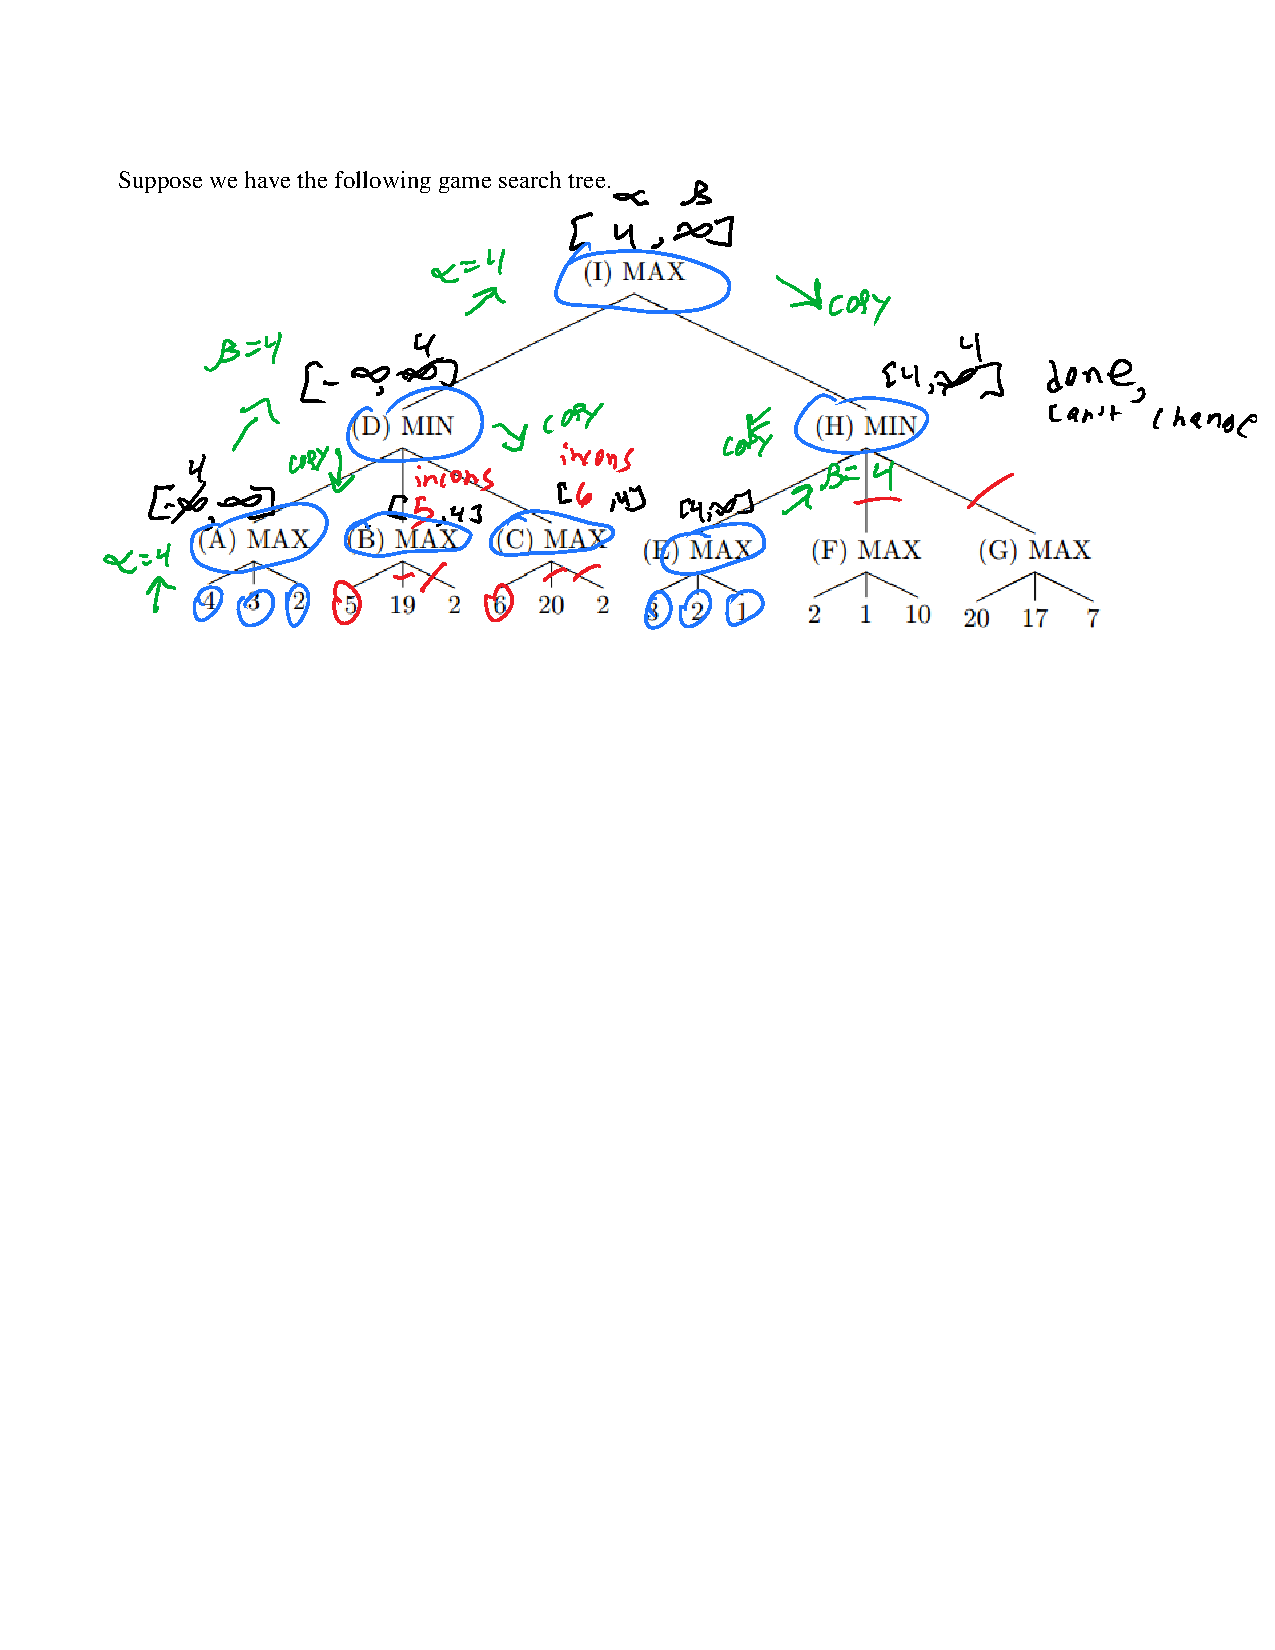
\includegraphics[width=.19\textwidth]{abprun.pdf}
\\ Local beam search with $k=1$ $\to$ hill climbing. LBS with 1 init
state and return as many as possible $\to$ BFS. SA with $T=0 \to $ HC,
SA with $T=\infty \to$ rand walk.
\\ Knapsack prob, var for each item, domain is $\{0,1\}$ (in bag or
not), constraint is sum should be less than cap.
\\ Map of diff cities, 2 friends in diff cities, each wait for other,
only 1 new node at a time. Want to meet. States: pair of cities. Succ:
neighbor nodes. Cost: max dist of both friends.
%%% Local Variables:
%%% mode: latex
%%% TeX-master: "Midterm"
%%% End:

\end{multicols*}
\end{document}